
\section{Appendix: Segmentation Examples at Different Compression Ratios}
\label{appendix:segmentation}

We provide representative examples of how boundary prediction behaves under different compression ratios across three content types: casual English text, Python code, and mathematical exposition.

\subsection{Casual English Text}

\textbf{Original (90 tokens):}
\begin{quote}
\small
So I've been trying to perfect my morning coffee routine lately. It's funny how something so simple can have so many variables. I started with a basic drip machine, which was fine, but a bit boring. Then I went down the French press rabbit hole – way more flavor, but the cleanup is a real hassle, you know?
\end{quote}

\textbf{Compression 8× (11 segments):}
\begin{quote}
\small
So I | 've been trying to perfect my morning coffee routine lately. | It's funny how something | so simple can have so many variables. | I started with | a basic drip machine, which | was fine, but a | bit boring. | Then I went down the French press rabbit hole – | way more flavor, but the cleanup is a | real hassle, you know?
\end{quote}

\textbf{Compression 4× (35 segments):}
\begin{quote}
\small
So I | 've been trying | to perfect | my morning coffee routine lately. | It's | funny how something | so simple can | have so many variables. | I started | with | a basic drip machine, which was fine, but | a bit boring.
\end{quote}

\textbf{Compression 2× (56 segments):}
\begin{quote}
\small
So I | 've | been trying to | perfect | my | morning coffee routine | lately. | It | 's funny how | something so | simple | can | have so many | variables.
\end{quote}

\subsection{Python Code}

\textbf{Original (87 tokens):}
\begin{verbatim}
import torch
from torch.utils.data import Dataset, DataLoader
class SimpleTextDataset(Dataset):
    """A simple dataset for loading text data."""
    def __init__(self, texts, tokenizer, max_length=128):
        self.texts = texts
        self.tokenizer = tokenizer
\end{verbatim}

\textbf{Compression 8× (12 segments):}
\begin{verbatim}
import torch | from torch.utils.data import Dataset, DataLoader | 
class SimpleTextDataset(Dataset): | 
"""A simple dataset for loading text data.""" | 
def __init__(self, texts, tokenizer, max_length=128): | 
self.texts = | texts | self.tokenizer = | tokenizer
\end{verbatim}

\textbf{Compression 4× (29 segments):}
\begin{verbatim}
import torch | from torch.utils.data | import Dataset | , DataLoader | 
class Simple | TextDataset(Dataset): | """ | A | simple dataset for | 
def | __init__(self, texts, tokenizer, max_length= | 128): | 
self.texts = | texts
\end{verbatim}

\textbf{Compression 2× (58 segments):}
\begin{verbatim}
import | torch | from torch.utils.data import | Dataset, | DataLoader | 
class | Simple | TextDataset(Dataset): | """ | A simple | dataset for | 
def | __init__(self, | texts, | tokenizer | , | max_length= | 128): | 
self | .texts | = | texts
\end{verbatim}

\subsection{Mathematical Text}

\textbf{Original (95 tokens):}
\begin{quote}
\small
Euler's formula is a mathematical formula in complex analysis that establishes the fundamental relationship between the trigonometric functions and the complex exponential function. The formula states that for any real number x, $e^{ix} = \cos(x) + i\sin(x)$, where e is the base of the natural logarithm, i is the imaginary unit.
\end{quote}

\textbf{Compression 8× (13 segments):}
\begin{quote}
\small
Euler's formula is a | mathematical formula in complex analysis that establishes | the fundamental relationship between the trigonometric functions and the complex exponential function. | The formula states that | for any real number x, $e^{ix}$ = | $\cos(x) + i\sin(x)$, | where e | is the | base of the natural logarithm, i is the | imaginary unit
\end{quote}

\textbf{Compression 4× (32 segments):}
\begin{quote}
\small
Euler's | formula is | a mathematical formula in | complex analysis that establishes | the fundamental relationship between | the trigonometric functions and the | complex exponential function. | The formula states | that for any | real number x | , $e^{ix}$ = | $\cos(x) + i\sin(x)$, | where e | is | the base of the natural logarithm
\end{quote}

\textbf{Compression 2× (61 segments):}
\begin{quote}
\small
Euler | 's | formula is | a | mathematical formula | in | complex analysis that | establishes | the fundamental relationship between | the trigonometric functions | and | the complex exponential | function. | The | formula states | that | for | any | real number x | , | $e^{ix}$ = | $\cos(x)$ | + | $i\sin(x)$,
\end{quote}

\begin{figure}[h]
\centering
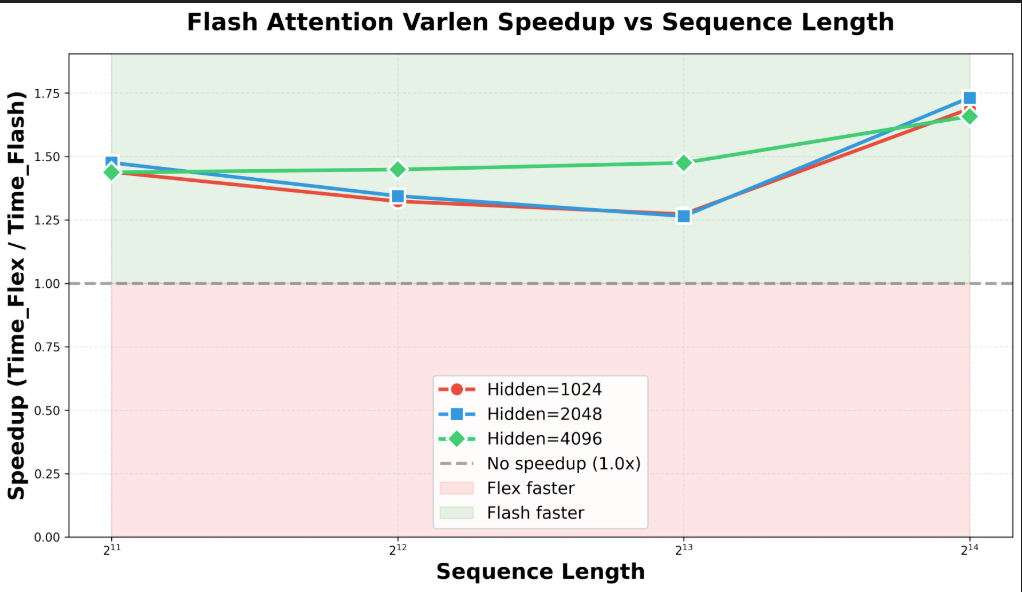
\includegraphics[width=0.9\textwidth]{speed_comp.png}
\caption{Flash Attention Varlen speedup ($T_{\text{flex}} / T_{\text{flash}}$) vs. Sequence Length. The plot visualizes the data from Table~\ref{tab:perf_comparison}, highlighting the performance trend across different scales and hidden sizes.}
\label{fig:speedup_plot}
\end{figure}

\begin{table}[h]
\centering
\caption{Performance comparison (Batch=1, Heads=32, Interval=6)}
\label{tab:perf_comparison}
\begin{tabular}{@{}ccccc@{}}
\toprule
Seq Length & Hidden Size & Flex (ms) & Flash Varlen (ms) & \textbf{Speedup} \\
\midrule
2048  & 1024 & 32.35 & 22.48 & \textbf{1.44$\times$} \\
2048  & 2048 & 33.31 & 22.58 & \textbf{1.48$\times$} \\
2048  & 4096 & 32.42 & 22.56 & \textbf{1.44$\times$} \\
\midrule
4096  & 1024 & 59.75 & 45.15 & \textbf{1.32$\times$} \\
4096  & 2048 & 60.72 & 45.17 & \textbf{1.34$\times$} \\
4096  & 4096 & 65.88 & 45.48 & \textbf{1.45$\times$} \\
\midrule
8192  & 1024 & 116.35 & 91.42 & \textbf{1.27$\times$} \\
8192  & 2048 & 114.65 & 90.66 & \textbf{1.26$\times$} \\
8192  & 4096 & 142.75 & 96.79 & \textbf{1.47$\times$} \\
\midrule
16384 & 1024 & 314.35 & 186.21 & \textbf{1.69$\times$} \\
16384 & 2048 & 323.53 & 186.83 & \textbf{1.73$\times$} \\
16384 & 4096 & 315.69 & 190.38 & \textbf{1.66$\times$} \\
\bottomrule
\end{tabular}
\end{table}
